\section{Black box modeling approach}

% Motivation for a black box model of the complete circuit
The goal of the black-box modeling method is to build a combined electrical and failure model of an integrated function between an input pin and an output pin.
This model is developed to allow third-parties that don't have access to the integrated circuit design to perform ESD simulations of a board containing integrated circuits.
Basically, this black box model is intended to act as a replacement for the \gls{ic} function during \gls{esd} board-level simulations.
This combined system-level and integrated circuit simulation approach is very valuable for designing robust applications, and is almost identical to the \gls{seed} \cite{seed} methodology introduced in previous chapters.
The \gls{seed} methodology normally applies to hard-failure, but in this chapter the concept is pushed further with soft-failures.
\gls{seed} recommends that the ESD robustness of a system should be handled by a collaboration between the board and the integrated circuit.
To achieve this, it is necessary to have simulation tools capable of simulating both elements at the same time.
The black-box model presented in this chapter is a potential solution to this issue.
It does not reveal the internal IC design while allowing complete simulations of board and integrated circuits together to predict soft-failures.
It also hides the internal complexity of the integrated circuit design, allowing significantly faster simulations and less convergence issues.

% Explanation of the model
The proposed model is composed of two port models and a failure model as shown in Fig. \ref{fig:black-box-principle}.
The electrical parts enable \gls{spice} simulations with this model inside an electrical environment.
The port model reproduces the behavior of the integrated circuit between an external pin and usually a ground pin.
The failure part of the model watches the external input pin and detects conditions that would lead to a failure visible on the external output pin.
If a fail was detected, the information is transferred to the output port model that will reproduce the behavior of the output during a failure.

\begin{figure}[!h]
  \centering
  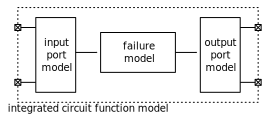
\includegraphics[width=0.65\textwidth]{src/4/figures/black_box_model_principle.pdf}
  \caption{Black-box model principle}
  \label{fig:black-box-principle}
\end{figure}

% How is the model constructed
The failure model is obtained with a preliminary characterization method.
It is also inspired by the Wunsch-Bell methodology \cite{wunsch-bell}.
The failure model is extracted first, using a set of rectangular pulses of variable amplitudes and variable widths applied on the input pin while monitoring the output pin.
After this step, the robustness of the function against this range of stresses is known.
A curve is built that describes the failure of the output when an input is stressed.
The second step is to electrically model both the input and the output ports.
Initially, a \gls{tlp} characterization of each port is performed to extract an equivalent I(V) curve.
Since the circuit is stressed while being powered and in operation, it is studied afterward if this extraction should occur on a device powered as well or not, and what is the impact of the supply on the extracted curve.
This characterization is based on the hypothesis that the quasi-static I(V) curve could be suitable for reproducing the behavior of the port both in DC and transient domain.
It will be demonstrated afterward that this hypothesis is not completely true and an alternative approach is required for the output pin.
This I(V) curve is converted in an electrical model using a piecewise-linear curve described in Verilog-A modeling language.
Finally, once the two electrical models and the failure model have been constructed, it can be possible to join all the parts together to build the complete IC model.

% What is the case study
To validate the concept, the characterization is performed on the integrated primary supply studied earlier (see Chapter \ref{sec:supply-desc}).
The input pin is called $V_{batt}$ and accepts the battery supply voltage.
The output pin is called $V_{2p5}$ and is supposed to deliver a \SI{2.5}{\volt} regulated supply.
Fig. \ref{fig:black-box-applied} summarizes the model configuration with those pins and function.

\begin{figure}[!h]
  \centering
  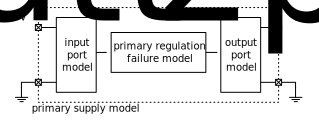
\includegraphics[width=0.65\textwidth]{src/4/figures/black_box_model_applied.pdf}
  \caption{Black-box model applied to the primary regulation function}
  \label{fig:black-box-applied}
\end{figure}


\subsection{Function failure model}

% First the function failure is characterized
The primary regulation function is characterized by applying a set of rectangular pulses of variable widths and variable amplitudes on the input pin, while monitoring the behavior of the output pin.
In case of significant variations of behavior, a failure is recorded.
The characterization yields a lookup table (see Table \ref{tab:cz-failure}) that associates to an input width and an input amplitude a flag representing the presence or absence of a failure.

\begin{table}[!h]
\centering
\begin{tabular}{@{}lll@{}}
\toprule
input width (ns) & input amplitude (V) & Failure   \\ \midrule
10               & 1                   & No        \\
10               & 2                   & No        \\
etc.             & ...                 & ...       \\
100              & 1                   & No        \\
etc.             & ...                 & ...       \\
1000             & 10                  & Yes       \\
etc.             & ...                 & ... \\ \bottomrule
\end{tabular}
\caption{Example of resulting table of failure characterization}
\label{tab:cz-failure}
\end{table}

% How is the characterization conducted and with which values
The characterization pulses are injected on the $V_{batt}$ input.
If a voltage below \SI{2.1}{\volt} is detected on $V_{2p5}$, a failure is recorded.
This voltage threshold is the failure criteria.
This value was chosen because it corresponds to a level below which digital cells powered by this supply will have noise margins too small for proper operation.
The input stress amplitude range is \SIrange{-50}{-500}{\volt}.
The input stress width is comprised between \SI{1}{\nano\second} and \SI{1000}{\nano\second}.
The characterization setup is given in Fig. \ref{fig:cz-black-box-setup}.
On the input pin, a \SI{12}{\volt} bias supply is connected in series with the rectangular pulse generator.
On the output, a \SI{100}{\nano\farad} capacitor is connected because required by the voltage regulation function for stabilization.

\begin{figure}[!h]
  \centering
  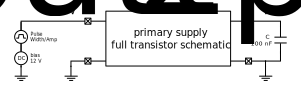
\includegraphics[width=0.7\textwidth]{src/4/figures/black_box_model_setup.pdf}
  \caption{Black-box characterization setup}
  \label{fig:cz-black-box-setup}
\end{figure}

% Detail the characterization
The result of the characterization is plotted in Fig. \ref{fig:cz-black-box}.
The x-axis is the pulse width, the y-axis is pulse amplitude and a colored cell represents a failure on the output.
This plot is simply a different representation of the lookup table discussed previously.
The plot shows that a combination of long stresses and large amplitude are the most disturbing for the function.
Amplitude or width alone are not necessarily sufficient to put the function at fault.

\begin{figure}[!h]
  \centering
  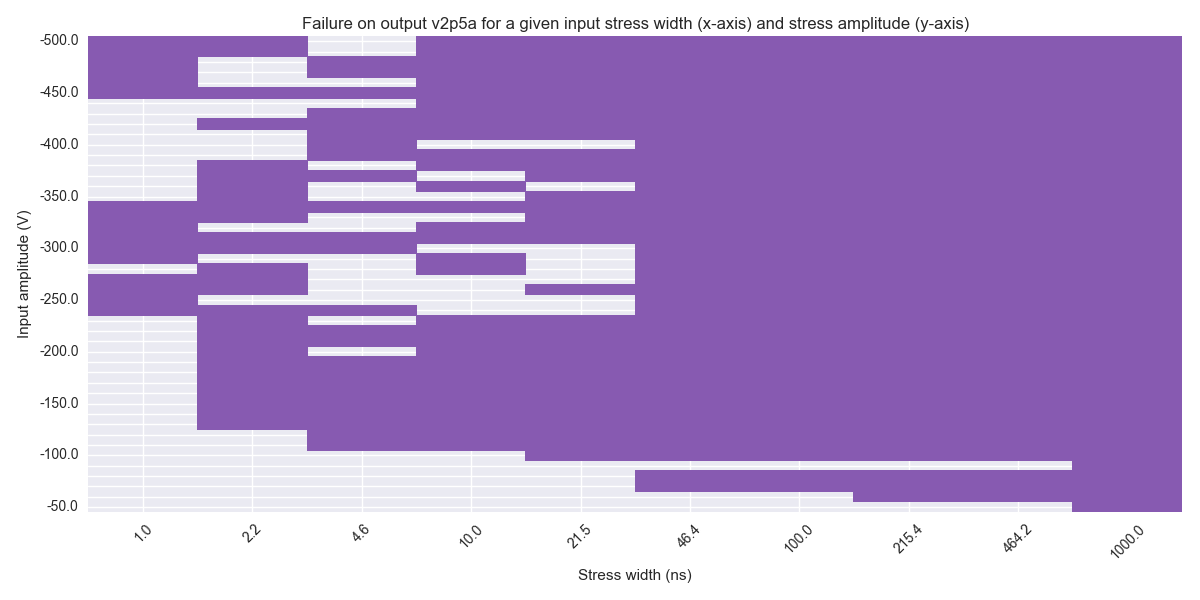
\includegraphics[width=\textwidth]{src/4/figures/black_box_regulator.png}
  \caption{Black-box characterization of the regulation function (cases in grey correspond a failure and transparent cases to no-failure.)}
  \label{fig:cz-black-box}
\end{figure}

Now that the characterization step is done, the next part of this work focuses on electrical modeling of input and output pins.

\subsection{Electrical pin models}
\subsubsection{I(V) curve extraction in powered and unpowered modes}

% Choose between powered or unpowered conditions
The initial hypothesis in this section is that \gls{tlp} characterization can be used to represent an input or output port of an integrated function.
Extracting the \gls{tlp} characteristic can be done with the device powered or unpowered.
To see the impact of the biasing and decide the best approach, \gls{tlp} characterizations are performed in both conditions.
The test setup for the input port is given in Fig. \ref{fig:tlp-input-testbench}.
The DC source can be configured at \SI{0}{\volt} (unpowered conditions) or \SI{12}{\volt} (powered conditions).
The TLP is a perfect rectangular source in combination with a series \SI{50}{\ohm} resistor.

\begin{figure}[!h]
  \centering
  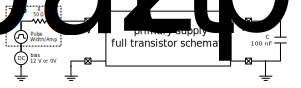
\includegraphics[width=0.8\textwidth]{src/4/figures/black_box_model_tlp_setup.pdf}
  \caption{I(V) extraction of input port}
  \label{fig:tlp-input-testbench}
\end{figure}

The test setup for the output port is given in Fig. \ref{fig:tlp-output-testbench}.
The main issue with this characterization is that it includes the external stabilization capacitor.
It will be verified after if this external device is an issue for modeling.
The results are provided for the input and output ports in Fig. \ref{fig:tlp-input-cz} and \ref{fig:tlp-output-cz}.

\begin{figure}[!h]
  \centering
  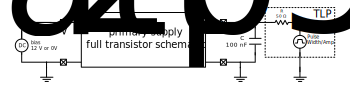
\includegraphics[width=0.9\textwidth]{src/4/figures/black_box_model_tlp_setup_output.pdf}
  \caption{I(V) extraction of output port}
  \label{fig:tlp-output-testbench}
\end{figure}

\begin{figure}[!h]
  \centering
  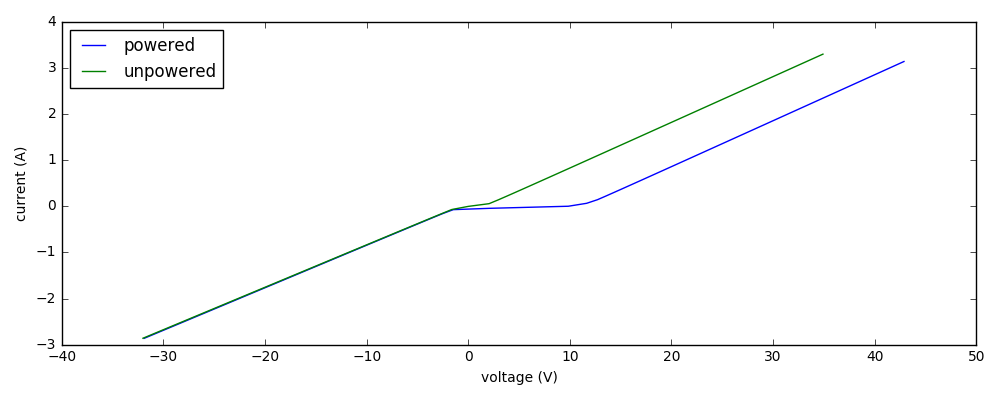
\includegraphics[width=\textwidth]{src/4/figures/tlp_input_characterization.png}
  \caption{TLP characterization of function input in powered and unpowered conditions}
  \label{fig:tlp-input-cz}
\end{figure}

\begin{figure}[!h]
  \centering
  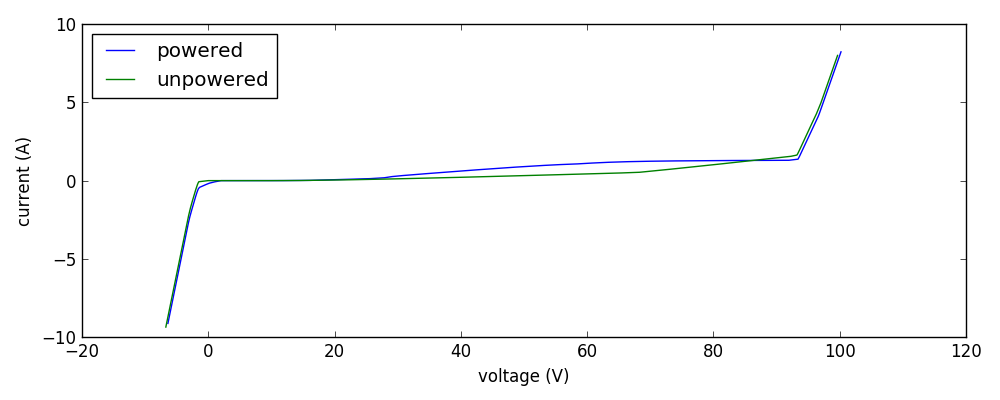
\includegraphics[width=\textwidth]{src/4/figures/tlp_output_characterization.png}
  \caption{TLP characterization of function output in powered and unpowered conditions}
  \label{fig:tlp-output-cz}
\end{figure}

% Comment the results
For both ports, large differences are observed between powered and unpowered modes.
Different amount of currents are absorbed by the device in each conditions.
Ultimately, the powered configuration is chosen for the characterization because it is the one used for soft-failure testing (with the device in operation).

\subsubsection{I(V) curve modeling}

% Explain the PWL model
The second step of the modeling method is to build an electrical model of the function from those curves.
A piecewise linear model seems well suited for this situation.
A four-points piecewise linear model is written in Verilog-A (see Listing \ref{lst:pwl-4pts}).
The model is configured easily with 4 four (V\textsubscript{i},I\textsubscript{i}) coordinates.

\begin{code}
\inputminted[frame=single]{verilog}{src/4/snippets/pwl_4pts.va}
\caption{Piecewise linear 4-points Verilog-A model}
\label{lst:pwl-4pts}
\end{code}

% How to avoid convergence issues
With this kind of model, convergence can be difficult to achieve if the piecewise-linear curve is not continuous at order 0.
Electrically speaking, it is equivalent to switching the value of a resistor very abruptly.
To ensure that this does not happen, it is important to use \textbf{exactly} the same coordinates at inflexion points, where the model switches between operating curves.
This is taken into account in the current model.

% Focus on the area of interest
During this \gls{tlp} characterization, I(V) curves were extracted for a wide range of voltages.
However, not the entire I(V) curve is relevant for those soft-failure simulations.
Any part of the I(V) curve beyond the safe operating area is irrelevant because after that the function is destroyed.
Therefore, it is important to fit the I(V) curve with the piecewise linear curve inside the SOA.
For the input, the modeling is focused on a voltage range from \SIrange{-10}{40}{\volt}.
On the output, the modeling range is from \SIrange{-5}{5}{\volt}.
Those values are obtained from the function specification and correspond to the sustained input ranges.

\subsubsection{Comparison of input model with reference circuit}

% Validate the model with TLP
The Verilog-A model is tested against the complete schematic for the function's input.
The test setup is given in Fig. \ref{fig:compare-veriloga-model-input}.
Biasing and injection circuits are identical for both circuits.
The full schematic is simply replaced by the Verilog-A input model.

\begin{figure}[!h]
  \centering
  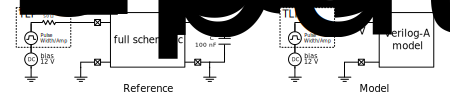
\includegraphics[width=0.95\textwidth]{src/4/figures/testbench_blackbox_input.pdf}
  \caption{Testbench for comparing complete schematic with input model simulations}
  \label{fig:compare-veriloga-model-input}
\end{figure}

% What is the result of comparison of model versus complete schematic for input ?
A first comparison is ran by injecting a \SI{-10}{\volt} TLP with the device powered.
The voltage and current waveforms are provided in Fig. \ref{fig:compare-model-simu-m10}.
Voltage matches well between the reference and the Verilog-A model.
The DC behavior as well as the transient behavior are correctly reproduced.
The current waveform has a poorer correlation.
There is an offset in DC and in transient, probably due to a modeling error with the piecewise linear curve.
There are two large spikes at the beginning and the end of the pulse that are not reproduced.
This behavior was expected because the piecewise-linear model is not able to reproduce this kind of dynamic behavior.
Overall, the accuracy remains acceptable for an ESD simulation.
Other validations are provided for positive \SI{20}{\volt} and \SI{40}{\volt} TLP in Fig. \ref{fig:compare-model-simu-20} and Fig. \ref{fig:compare-model-simu-40}).
They confirm that the input model performs correctly, and even better when exposed to positive stresses.
Overall, this Verilog-A model is considered valid for the input port while considering that there is a lot of room for improvement.

\begin{figure}[!p]
  \centering
  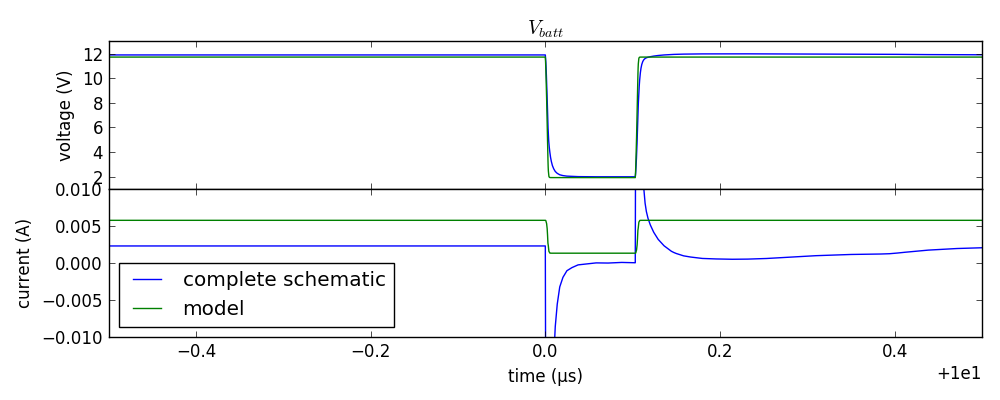
\includegraphics[width=0.8\textwidth]{src/4/figures/comparison_model_total_m10V.png}
  \caption{Comparison of complete schematic and model simulations for input port (\SI{-10}{\volt} TLP)}
  \label{fig:compare-model-simu-m10}
\end{figure}

\begin{figure}[!p]
  \centering
  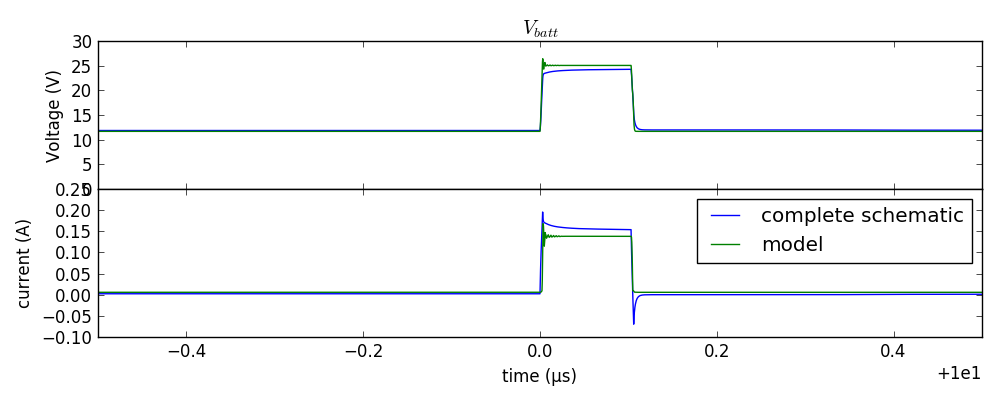
\includegraphics[width=0.8\textwidth]{src/4/figures/comparison_model_total_20V.png}
  \caption{Comparison of complete schematic and model simulations for input port (\SI{20}{\volt} TLP)}
  \label{fig:compare-model-simu-20}
\end{figure}

\begin{figure}[!p]
  \centering
  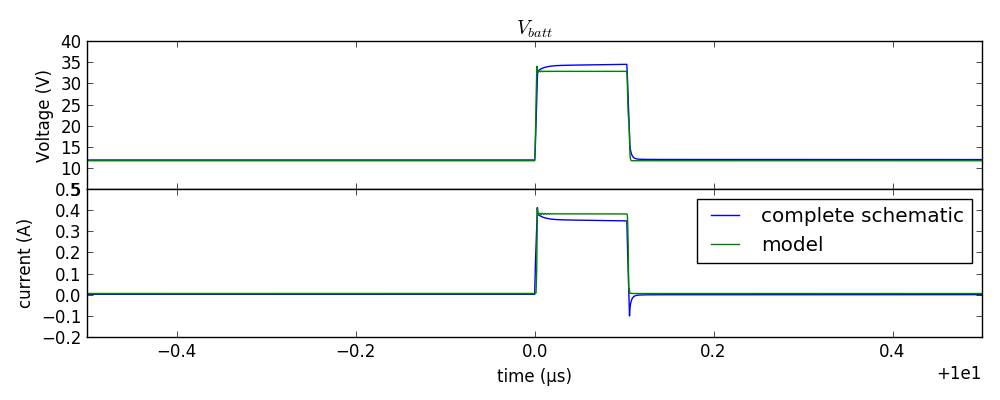
\includegraphics[width=0.8\textwidth]{src/4/figures/comparison_model_total_40V.png}
  \caption{Comparison of complete schematic and model simulations for input port (\SI{40}{volt} TLP)}
  \label{fig:compare-model-simu-40}
\end{figure}

\subsubsection{Comparison of output model with reference circuit}

% The output port is not a passive device
The output port is more complicated than the input port, because it is equivalent to an active device, unlike the input that can be assimilated to a passive port.
The primary supply regulates a \SI{2.5}{\volt} voltage on this output and drives a current into the external load to maintain that voltage.
The Verilog-A I(V) model used for the input is just a voltage controlled current source and is not capable of regulating a voltage.
A more complex architecture is proposed with Fig. \ref{fig:first-output-model}.
A DC voltage source is added to generate the regulated \SI{2.5}{\volt}.
In case of failure, the output port will also fail temporarily and the output voltage will fall down.
A transient voltage source is added to the model to simulate the output fault.

\begin{figure}[!h]
  \centering
  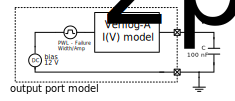
\includegraphics[width=0.7\textwidth]{src/4/figures/first_output_model.pdf}
  \caption{Architecture of the output port model}
  \label{fig:first-output-model}
\end{figure}

% Make the comparison
This new output port model is compared to the complete schematic in simulation.
With the complete schematic, a failure is triggered by applying a negative \SI{-10}{\volt} TLP on the input port $V_{batt}$ while watching the output $V_{2p5}$.
For the model, the PWL source is used to fake a failure.
The testbench is identical to the input validation testbench shown previously (Fig. \ref{fig:compare-veriloga-model-input}).
Voltage and current waveforms are compared in Fig. \ref{fig:compare-model-simu-m10-output}.

\begin{figure}[!h]
  \centering
  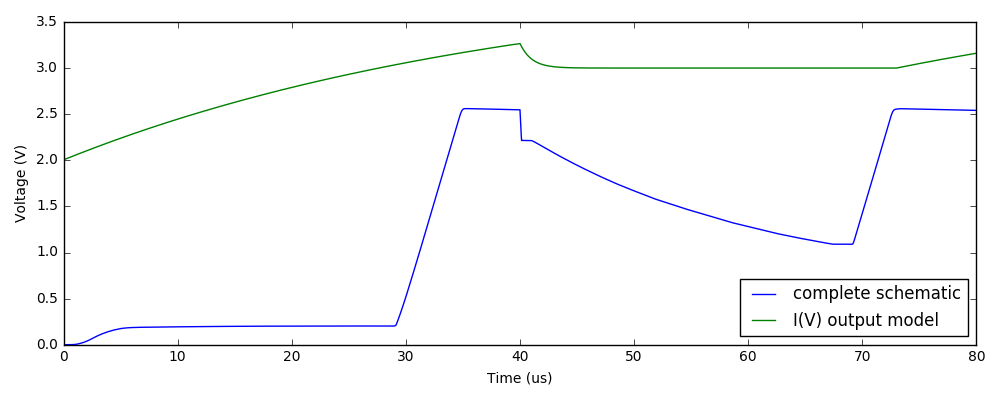
\includegraphics[width=\textwidth]{src/4/figures/comparison_model_total_output_bad_m10V.png}
  \caption{Comparison of complete schematic and model simulations for output port (\SI{-10}{\volt} TLP)}
  \label{fig:compare-model-simu-m10-output}
\end{figure}

% Comment the reference curve
Large differences are observed between reference and model simulations.
In the reference curve (in blue), the regulation function starts up between \SI{0}{\micro\second} and \SI{35}{\micro\second}.
This part of the curve is not particularly relevant for the ESD analysis and can be ignored overall.
At \SI{40}{\micro\second} the pulse is injected on the input (not plotted), resulting in a fault on this output.
In turn, the reference curve exhibits the typical restart explained previously in chapter \ref{sec:failure-case-study}.
The voltage drops until \SI{1}{\volt}.
The regulator restarts until it is operating properly again at \SI{75}{\micro\second}.

% Comment the model curve
The model curve (in green) is very different from the reference.
Initially, the \SI{100}{\nano\farad} capacitor connected on the output (Fig. \ref{fig:first-output-model}) is pre-charged at \SI{2}{\volt}.
This value is voluntarily set at a lower value than the nominal \SI{2.5}{\volt} to ensure that the model alone is capable of reaching this DC operating point.
Instead of reaching and stabilizing at \SI{2.5}{\volt}, the output voltage keeps increasing.
This can be explained by looking at the I(V) curve of the output magnified between \SI{1}{\volt} and \SI{4}{\volt} (see Fig. \ref{fig:tlp-output-cz-zoomed}).
At the beginning of the simulation, the I(V) model sees a potential difference of \SI{2.0}{\volt} across its terminals.
For a \SI{2.0}{\volt} voltage, the I(V) curve model produces a value of \SI{0.75}{\milli\ampere}.
It is not identical to the characterized value of \SI{0.2}{\milli\ampere} but the error remains acceptable.
This non-zero current is therefore forced by the Verilog-A model into the capacitor, that keeps charging.
In itself, the combination of the DC source and the I(V) curve does not seem suitable for modeling an active output.

\begin{figure}[!h]
  \centering
  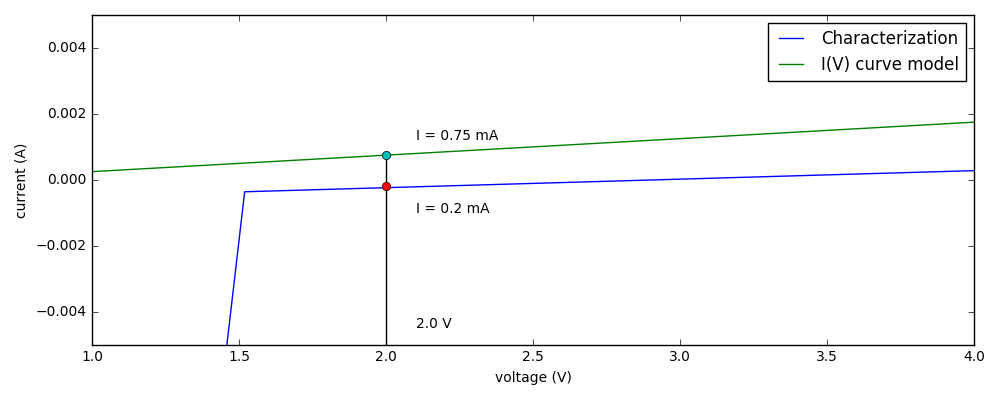
\includegraphics[width=\textwidth]{src/4/figures/tlp_output_characterization_magnified.png}
  \caption{TLP characterization of function output near \SI{2.5}{\volt} (magnified)}
  \label{fig:tlp-output-cz-zoomed}
\end{figure}

Configuring the Verilog-A model to generate a zero current at \SI{2.5}{\volt} will not solve the problem either because with a resistive load the output will need to supply a DC current at \SI{2.5}{\volt}.
The I(V) curve extracted with a TLP characterization in simulation does not seem to be usable as-is to model an active output.
A more complex or different solution must be conceived and developed to solve those issues.
One potential solution would be to create a custom Verilog-A model capable of regulating a voltage while offering proper output impedance.
Overall, this study on input and output ports modeling has enabled to identify key issues preventing for now to develop a complete model of integrated function for powered ESD simulations.
This is a first step toward more advanced models and modeling techniques that ultimately should enable better cooperation between silicon-design companies and equipment manufacturers, as described by the SEED methodology.

\subsection{Conclusion on black-box modeling}


% Conclusion
Black box models are very promising for distributing SPICE models of integrated functions to third-parties without disclosing intellectual property.
They do not disclose the internal design of the chip and might help achieve system-level ESD simulations with IC models.
Ultimately, the goal is to follow the SEED \cite{seed} methodology that indicates that ESD robustness of a system should not be handled by a single component but with a collaboration between all parts (equipment, board, integrated circuit), using appropriate design techniques to ensure that the cooperation is efficient.
In this section, a first attempt at extracting and creating black-box models for integrated functions was presented, in the context of ESD simulations.
TLP characterization was performed on input and output pin of a biased function, to extract an equivalent impedance.
The resulting I(V) curve was then modeled using Verilog-A modeling language, then used in circuit simulations.
For the input pin that is somehow equivalent to a passive device, this model has shown promising results with excellent correlation in both DC and transient domains.
The Verilog-A model performed particularly well for the input when exposed to a positive rectangular stress.
The correlation was less accurate with a negative rectangular pulse but remained acceptable for an ESD simulation.
For the output pin, the situation was more complex because it should be modeled by an equivalent active device.
A first model was proposed specifically for modeling active outputs, however it was not successful.
Differences between the reference schematic and the model were simply too large, showing that a different or more complex approach is required.
Despite the lack of correlation, this study has enabled to identify an important issue preventing to build a model of an integrated function, for ESD simulations.
Solving this issue should be the topic for future work and research, and identifying it was already a significant milestone to reach for achieving this goal.
Ultimately, black box models should enable to replace an integrated function during an ESD simulation, in order to reduce complexity, simulation time, and protect intellectual property.

% Opening work
There are many new approaches to explore on these black box models to get more accurate results.
It was shown that modeling of active outputs directly with a \gls{tlp} characterization and a bias does not seem to work and more research is required on this topic.
Also, the behavior of the input port model against non-rectangular waveforms should be studied and investigated to ensure that the model works correctly in dynamic regime.
The piecewise-linear modeling technique, usually employed in the ESD field for modeling ESD protections, should be improved by adding more points to fit more closely the extracted I(V) curve.
Also, this methodology should be applied to a wider number of analog functions, to observe if it can be used in a general manner.
Research on all those topics should lead to the development of a black-box model that will work for powered electrostatic discharge simulations.
